\documentclass{article}

\usepackage[heading=true]{ctex}
\usepackage[backref]{hyperref}
\usepackage{filecontents}
\usepackage{float}
\usepackage{graphicx}
\usepackage{geometry}
\usepackage{dirtree}
\usepackage{listings}
\usepackage{xcolor}
\usepackage{qtree}

\ctexset{
    section={
        number=\chinese{section},
        format+=\raggedright
    }
}
\geometry{a4paper, scale=0.7}

\definecolor{codegreen}{rgb}{0,0.6,0}
\definecolor{codegray}{rgb}{0.5,0.5,0.5}
\definecolor{codepurple}{rgb}{0.58,0,0.82}
\definecolor{backcolour}{rgb}{0.98,0.98,0.98}

\lstdefinestyle{lststyle}{
    backgroundcolor=\color{backcolour},
    commentstyle=\color{codegreen},
    keywordstyle=\color{magenta},
    numberstyle=\tiny\color{codegray},
    stringstyle=\color{codepurple},
    basicstyle=\ttfamily\small,
    breakatwhitespace=false,
    breaklines=true,
    captionpos=b,
    keepspaces=true,
    numbers=left,
    numbersep=5pt,
    showspaces=false,
    showstringspaces=false,
    showtabs=false,
    tabsize=2
}

\lstset{style=lststyle}


\title{实验一: PyTorch实现MLP}
\author{1190200703 管健男}
\date{}


\begin{document}

\maketitle


\section{实验环境}

\subsection{软硬件环境}

\begin{table}[h]
    \centering
    \begin{tabular}{|c|c|}
        \hline
        \textbf{OS}      & Linux 5.17.4-arch1-1 x86\_64 GNU/Linux \\
        \textbf{Python}  & 3.10.4                                 \\
        \textbf{Pytorch} & 1.11.0+cu113                           \\
        \textbf{rustc}   & 1.60.0 (7737e0b5c 2022-04-04)          \\
        \hline
    \end{tabular}
    \caption{编译环境}
\end{table}

\begin{table}[h]
    \centering
    \begin{tabular}{|c|c|}
        \hline
        \textbf{CPU}        & 11th Gen Intel(R) Core(TM) i7-11700 @ 2.50GHz \\
        \textbf{GPU}        & NVIDIA GeForce RTX 3060 Lite Hash Rate        \\
        \textbf{GPU Driver} & 510.60.02                                     \\
        \textbf{CUDA}       & 11.6                                          \\
        \hline
    \end{tabular}
    \caption{硬件环境及驱动}
\end{table}

\subsection{源码目录结构}

源码目录结构如图\ref{src-dir}

\begin{figure}[H]
    \centering
    \begin{minipage}{0.5\linewidth}
        \dirtree{%
            .1 PatternRecognitionAndDeepLearningLabs.
            .2 DeepLearning.
            .3 lab1.
            .4 image-generator.
            .5 Cargo.lock.
            .5 Cargo.toml.
            .5 src.
            .6 main.rs.
            .4 model.
            .5 model.pt.
            .4 dataloader.py.
            .4 main.py.
            .4 model.py.
            .4 trainer.py.
            .2 report.
            .3 LD-lab1.
            .4 LD-lab1.pdf.
            .4 LD-lab1.tex.
        }
    \end{minipage}
    \caption{源码目录结构}
    \label{src-dir}
\end{figure}

要进行训练并保存模型,只需修改main.py中load\_model为False,并在
PatternRecognitionAndDeepLearningLabs/DeepLearning/lab1目录下
运行python main.py。

\begin{figure}[H]
    \centering
    \begin{minipage}{.7\textwidth}
        \centering
        \lstset{numbers=left,xleftmargin=2em,breaklines,language=Python, aboveskip=0pt,belowskip=0pt}
        \lstinputlisting[firstline=1,lastline=1,firstnumber=5]{load_model.py}
        \lstinputlisting[firstline=2,lastline=2,firstnumber=6,backgroundcolor=\color{orange!30}]{load_model.py}
        \lstinputlisting[firstline=3,lastline=4,firstnumber=7]{load_model.py}
    \end{minipage}
    \caption{训练新模型并保存}
\end{figure}

要直接使用已有模型,只需修改main.py中load\_model为True即可。

\begin{figure}[H]
    \centering
    \begin{minipage}{.7\textwidth}
        \centering
        \lstset{numbers=left,xleftmargin=2em,breaklines,language=Python, aboveskip=0pt,belowskip=0pt}
        \lstinputlisting[firstline=6,lastline=6,firstnumber=5]{load_model.py}
        \lstinputlisting[firstline=7,lastline=7,firstnumber=6,backgroundcolor=\color{orange!30}]{load_model.py}
        \lstinputlisting[firstline=8,lastline=9,firstnumber=7]{load_model.py}
    \end{minipage}
    \caption{测试现有模型}
\end{figure}

\section{实验内容}

\subsection{读取数据}

使用torchvision自带的MNIST数据集加载函数torchvision.datasets.MNIST,
可以自动下载缺失的数据集。
其返回dataloader数据格式为$[(x, y), (x, y), (x, y), ...]$,
其中$x$为数据,$y$为标签。
设置batch\_size参数可以指定每次读取的数据量,实验代码中设置为20。

\subsection{构建模型}

使用torch.nn.Linear构建输入层和隐藏层,其中输入层大小是$28 \times 28 = 784$,
因为每一张图片都是$28 \times 28$大小。隐藏层数手动设置为100。
在经过每一层后,使用leaky relu作为激活函数。

模型结构如图\ref{mlp-model}。

\begin{figure}[H]
    \centering
    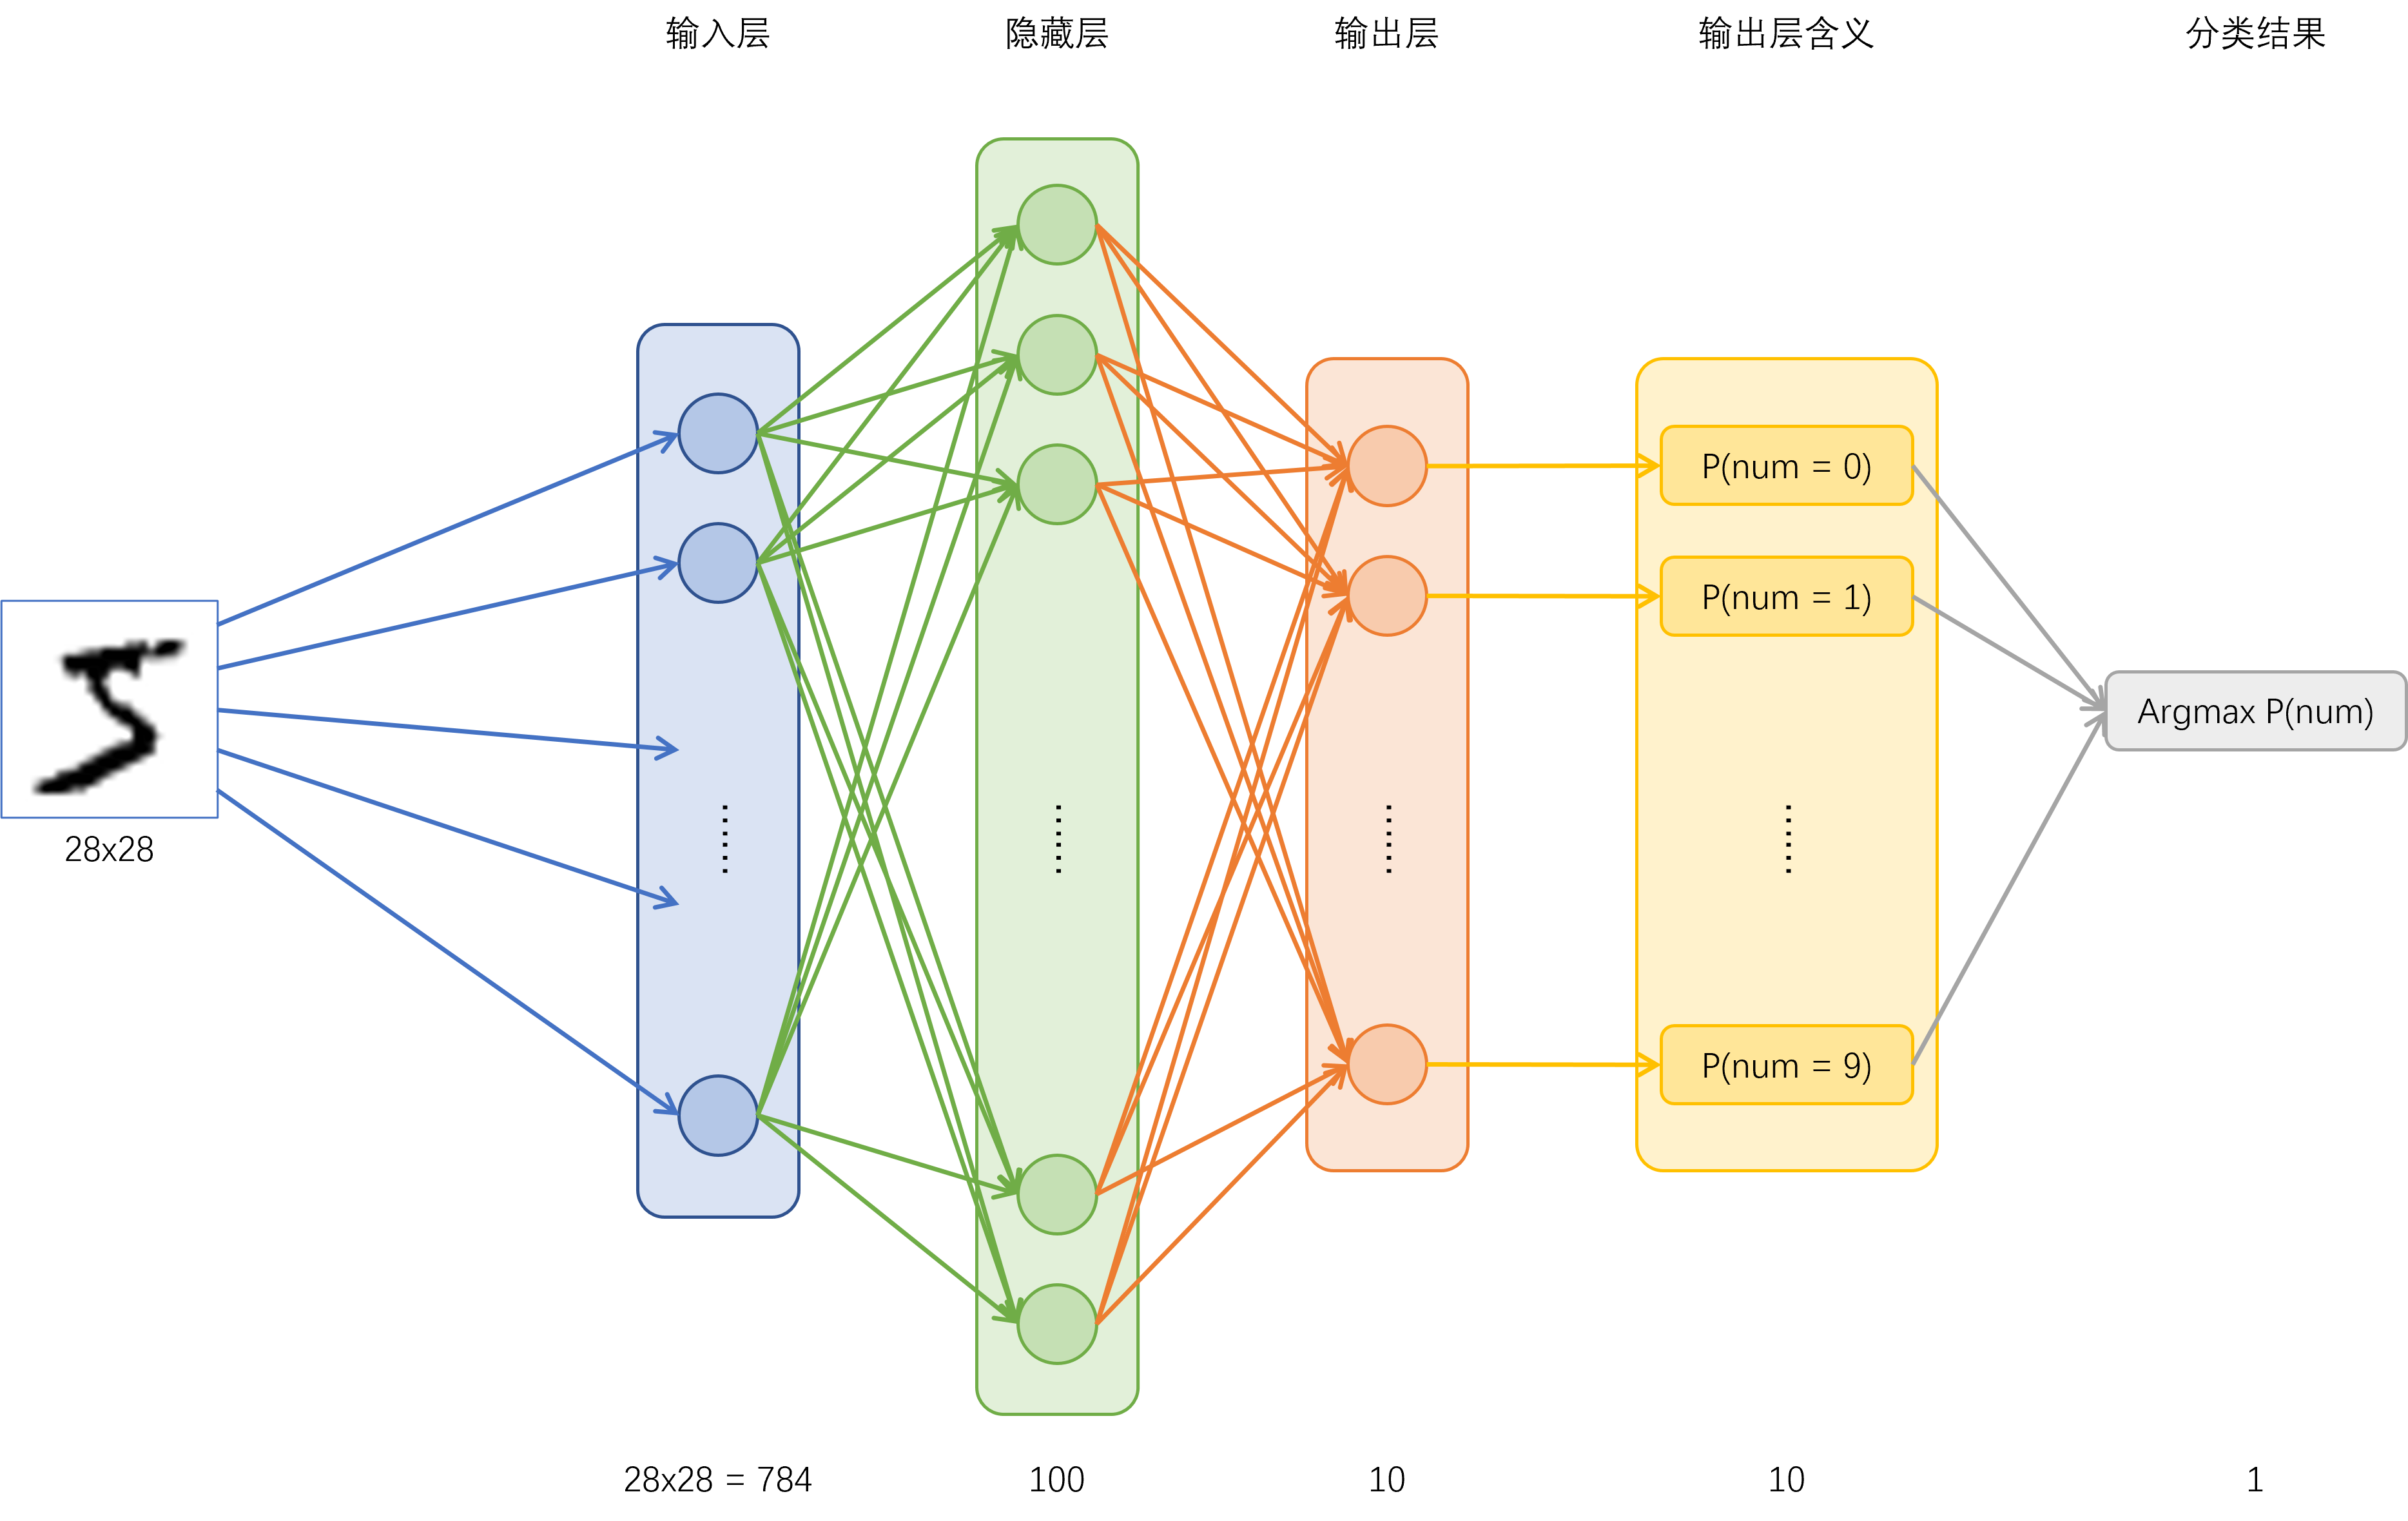
\includegraphics[width=\textwidth]{figures/fig_01.png}
    \caption{MLP模型结构}
    \label{mlp-model}
\end{figure}

模型的输出是一个10维向量(batch\_size=1时),表示手写数字图片是0到9的概率。
因此分类结果是这10个概率的最大值对应的数字号。

\section{实验结果与分析}

调整隐藏层特征数量,使其分别为5, 7, 10, 15, 20, 50, 100, 500,
训练次数epoch=20,数据批量batch\_size=20时绘制每次迭代的分类准确率,
如图\ref{hidden-features}所示。

\begin{figure}[H]
    \centering
    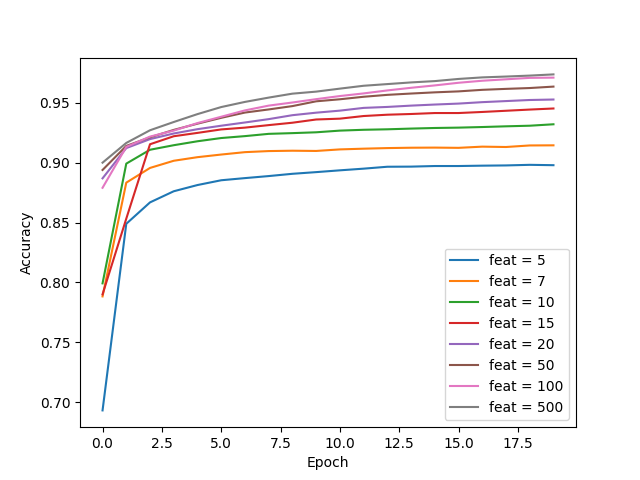
\includegraphics[width=0.8\textwidth]{figures/fig_02.png}
    \caption{隐藏层特征数分别为5, 7, 10, 15, 20, 50, 100, 500时的准确率}
    \label{hidden-features}
\end{figure}

经过实验,发现隐藏层特征越多,越有利于分类的准确率,但是当特征数大于100时,
准确率上升并不大,各个隐藏层特征数对应的分类准确率如图表\ref{hidden-features-acc}所示。

\begin{figure}[H]
    \begin{minipage}[H]{0.7\linewidth}
        \centering
        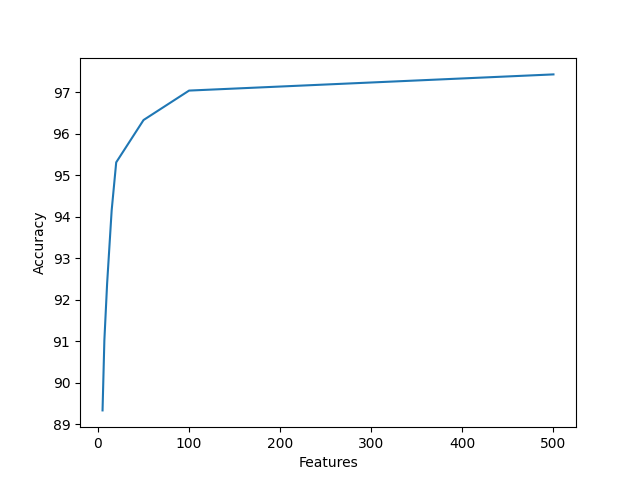
\includegraphics[width=\textwidth]{figures/fig_03.png}
    \end{minipage}
    \begin{minipage}[H]{0.2\linewidth}
        \centering
        \begin{tabular}{ll}
            \hline
            \textbf{Feat} & \textbf{Acc} \\
            \hline
            5             & 89.33\%      \\
            7             & 91.02\%      \\
            10            & 92.38\%      \\
            15            & 94.15\%      \\
            20            & 95.31\%      \\
            50            & 96.33\%      \\
            100           & 97.04\%      \\
            500           & 97.43\%      \\
            \hline
        \end{tabular}
    \end{minipage}
    \caption{各个隐藏层特征数对应的分类准确率}
    \label{hidden-features-acc}
\end{figure}

当隐藏层特征数量为500时,准确率可高达到97.43\%。
但是当特征数大于100之后,准确率随特征的上升已经不明显。

\end{document}
